\chapter[SCP-185 跨时空无线电]{
    SCP-185 The Radio\\
    SCP-185 跨时空无线电
}

\label{chap:SCP-185}

\begin{figure}[H]
    \centering
    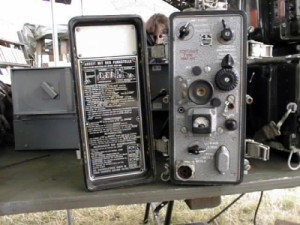
\includegraphics[width=0.5\linewidth]{images/SCP-185.jpg}
    \caption*{收容前的SCP-185}
\end{figure}

\bb{项目编号:}SCP-185

\bb{项目等级:}Safe(自从185-1事故发生之后,被考虑分级为Euclid级别。详情请阅185-1文档。)

\bb{特殊收容措施:}SCP-185目前被保存于一个隔音房间,房间内设置了多个具有噪音过滤功能的麦克风,以作监察之用。对于此项目需采取标准的保护措施。于房间内的所有人员必须佩戴护耳装备,测试者除外。

\bb{描述:}SCP-185是一部于冷战时期所应用的苏联R-105M无线电设备,特别的是,它加设了一块制作粗劣的键盘和液晶屏幕。绝大部份的无线电传输它都能够接收得到,包括一些经过加密处理的信号。一直以来,基金会都在尝试确认它是如何解读得到堪称世上最强的加密信号,可是到目前为止依然未有定论。SCP-185的信号接收范围极广,甚至比现今的无线电设备更为优越。它具有一般无线电装置的功能,但比较特别的是能够透过键盘向它输入信号。如果于键盘上输入一个年份的话,它就似乎能够接收得到来自该指定年代的信号(视乎这设定频率上有没有在进行信息广播)。这种功能是在随机键入一串数字──1939时被发现的,当时从装置中听到了内维尔·张伯伦\footnote{\bb{译注:}Neville Chamberlain,一位英国保守党政治家,在1937-40年间出任英国首相。}在向德国宣战。较早前察觉到于装置上输入精准时间和日期来进行实验的可能性,目前正在进行相关的研究。同时,现时亦正在讨论向其输入未来日期的可行性,但目前仍无法确法此举所带来的好处是否足以弥补产生时间悖论\footnote{\bb{译注:}原文为Time paradox,即是Temporal paradox,简单来说就是因控制或干扰时间流而导致时空产生混乱错误的情况。}的风险。无线电设备里面的布局并没有进行任何变动,而它的键盘则被收纳于一个固定在装备侧边的盒子里。这个盒子由一种未知金属所制作而成,用尽一切方法均无法对它进行切割或拆卸,所以目前研究人员并无法将键盘从盒子内分离出来。

\bb{附录:}

\bb{185-1文档:1号事故}

一次实验中,年份被设定为-137.3亿年,这年份处于宇宙诞生的估计时期之内。当时该物件所产生的声音并不能经由标准设备所检测得到。据事故中的生还者汇报,这是一种类似由太阳发射出的无线电波音频的隆隆声。所有处于声波震源方圆200米内的人皆因窒息而死,他们肺内的微细血管全都被这重声波所震破了。验尸报告指出,基本上所有受害者都是死于体内大量出血的。自从该事故之后,这件设备有时会操作失灵,亦发现设备的内部电池组件已经失效,经更换之后已恢复其正常功能。据报当时它的液晶屏幕仍是亮着的,不过相信除了上述的电池组件之外,装置并没有任何其他特殊的电力供应。该声波同时亦令到SCP-███无法正常运作,导致该SCP最终被无效化。事故当中该无线电设备似乎并无遭受任何损害。回报显示,事故现场遭受了结构性损害,迫使有关区域不得不停止运作以进行维修。此后,相关实验因而一直被无限期延长,直至另行通知为止。

\ii{「任何被抓到在执勤期间使用此物件来听音乐的人员均会遭受纪律处分。」}──\bb{████████博士}

\bb{项目使用申请:}

机动特遣队Delta-5分队申请应用SCP-185于他们的任务上,希望能抢先敌人一步追查目标对象。特遣队相信伊朗人手持着一些重要情报,希望能够以这设备截取到他们的通信信号。最后申请获得批准。
